%--------------------------------------------------------------------
\subsection{JACEK: Large-Scale Demonstration: NV Center in Diamond} 
\label{sec:nv}
%--------------------------------------------------------------------

As a final demonstration, we apply the periodic spin-polarized RT-TDDFT 
implementation to the negatively charged nitrogen-vacancy   (NV$^-$)
center in diamond, one of the most studied point defects in
solid-state physics.\cite{NV-Doherty-2013,NV-Gali-2008,NV-Gali-2019}%,nv-center-review}
The ground state of  NV$^-$ center is an optically addresable  spin-triplet located 
within  the diamond bad gap \cite{NV-Gali-2008,NV-Gali-2019,NV-Louie-2012}
Becasue of its optical adreasbility and long coherence times at room temperature the NV(-) center is 
an attractive system  for several emerging quantum technologies, including single -photon emitter,
nanoscale magnetometry, quantum sensing, quantum information 
processing.\cite{NV-coherence-Balasubramanian-2009,NV-sensing-Degen-2017,NV-sensing-Maze-2008,NV-sensing-Schirhagl-2014,NV-spe-Aharonovich-2016,NV-QComp-Bradley-2019}

This system tests several capabilities simultaneously: spin-polarized real-time propagation, 
optical response of a localized defect in a three-dimensional periodic host, 
convergence toward the dilute-defect limit, as well as  computational  scaling to  thousands of atoms 
The purpose of this section is not to provide a complete quantitative description of NV-photophysics.
%In particular, the experimental zero-phonon line (ZPL) involves vibronic structure, excited-state relaxation, and electron–phonon coupling, none of which are included in the fixed-ion calculations considered here. 
Instead, the present calculations examine the electronic optical response of defect in the energy region of 
the experimental zero-phonon line (ZPL) and use the NV$^-$ center to demonstrate how polarization selection rules,
periodic defect-image interactions, and active-space truncation affect large-scale periodic RT-TDDFT calculations.


    
\subsubsection{Electronic structure and  simulation setup for NV$^-$}


\begin{figure}[ht!]
	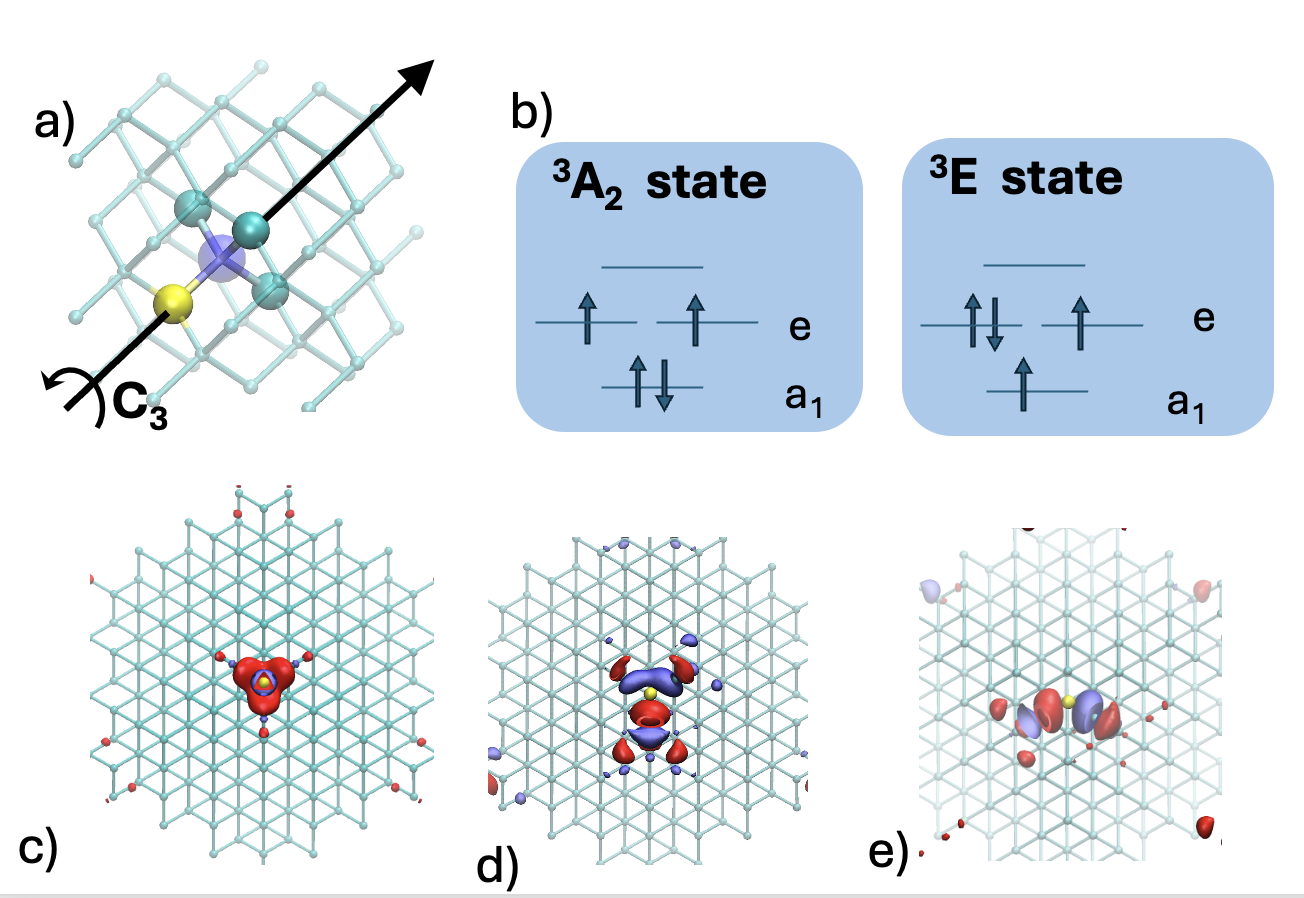
\includegraphics[width=0.5\columnwidth]{Figs/Figure-NV-center.png}
	\caption{\footnotesize
        Electronic structure of the negatively charged nitrogen-vacancy (NV$^-$) center in diamond.  
	(a) Local atomic structure of the defect, consisting of a substitutional nitrogen atom (green)  adjacent to a carbon vacancy (blue transparent). 
	The black arrow indicates the $[111]$ direction, which defines the $C_3$ symmetry axis of the approximately $C_{3v}$ defect environment.
	(b) Schematic occupation of the defect levels in the triplet ground state, ${}^3A_2$ (configuration $a_1^2 e_1^1 e_2^1$),
	and in the optically excited triplet ${}^3E$ state (configuration $a_1^1 e_1^2 e_2^1$),.
%	In the ground state, the lower $a_1$-like defect orbital is doubly occupied, while the two components of the $e$ manifold are
%	singly occupied with parallel spins (configuration $a_1^2 e_1^1 e_2^1$) and total spin $S=1$. 
	The defect-associated optical transition in the experimental zero-phonon-line energy region is dominated by promotion 
	of a minority-spin electron from the occupied $a_1$-like defect orbital into the $e$ manifold.
	(c--e) Representative real-space isosurfaces of Kohn--Sham defect orbitals localized in the diamond band gap (view along the C$_3$ axis: 
	(c) the occupied $a_1$-like orbital and 
	(d,e) the two components of the nearly degenerate $e$ manifold. Red and blue isosurfaces denote opposite
	phases of the Kohn--Sham orbitals.
        }
\label{fig:nv-structure}
\end{figure}

The NV$^-$ center consists of a substitutional nitrogen atom adjacent
to a carbon vacancy, with one additional electron trapped at the
defect (Figure~\ref{fig:nv-structure}a). The defect axis is oriented along the
crystallographic $[111]$ direction, which defines the $C_3$ symmetry
axis of the approximately $C_{3v}$ local defect environment. The
defect states are located within the diamond band gap. The lower
$a_1$-like defect orbital has substantial nitrogen character together
with contributions from the three carbon atoms adjacent to the vacancy,
whereas the nearly degenerate $e$ manifold is primarily localized on
these three carbon atoms, as shown in Figure~\ref{fig:nv-structure}c--e. Because
pristine diamond has a wide band gap of about 5.5~eV and is transparent
throughout the visible range, optical absorption and emission below
this energy arise from defect states; for NV$^-$, the
${}^3A_2 \rightarrow {}^3E$ transition has an experimental
zero-phonon line at 1.945~eV, corresponding to 637~nm red light.




All NV$^-$ calculations were performed here with the \texttt{RMG} code using
periodic boundary conditions, the PBE exchange-correlation functional,
and the \texttt{NC\_accuracy} norm-conserving pseudopotentials.  The
diamond lattice constant was first optimized for bulk diamond using the
same functional and pseudopotentials, giving
$a=3.5725125$~\AA.  This optimized lattice constant was then kept fixed
for all NV$^-$ defect calculations.

Three single-defect supercell sizes were considered, denoted NV-$x2$ (small),
NV-$x4$ (medium), and NV-$x8$ (large). These systems were constructed from
$2\times2\times2$, $4\times4\times4$, and $8\times8\times8$
repetitions of the conventional face-centered cubic (fcc) diamond cell, 
corresponding to 64, 512, and 4096 diamond lattice sites before formation of the defect.
%In each case, an NV$^-$ center was created by replacing one carbon atom
%with nitrogen and removing a nearest-neighbor carbon atom along the
%$[111]$ direction.  Therefore, 
Previous supercell studies of NV$^-$ in diamond have shown that
relatively large cells, on the order of the 512-site NV-$x4$ model,
are needed to reduce spurious interactions between periodic defect
images.\cite{NV-Gali-2008,NV-Gali-2019,NV-Louie-2012}  Here we
directly test this finite-size behavior by extending the real-time
calculations to the 4096-site NV-$x8$ cell.  The same 4096-site host
also enables explicit simulations of periodic arrays of NV$^-$ centers,
including collinear parallel and antiparallel defect-spin arrangements,
which are used below as an additional demonstration of spin-resolved
periodic RT-TDDFT.
The actual defect supercells contained
63, 511, and 4095 atoms, respectively.  The negatively charged
supercells were treated using a uniform compensating background charge
to maintain overall charge neutrality under periodic boundary
conditions.

The real-space grid was scaled with the supercell size so that all
three calculations used the same grid spacing.  The NV-$x2$, NV-$x4$,
and NV-$x8$ systems used $48^3$, $96^3$, and $192^3$ grid points,
respectively, corresponding to a grid spacing of $0.281\,a_0$.  
This grid corresponds to equivalent wavefunction and
charge-density cutoffs of 124.7 and 498.9~Ry, respectively; the
charge-density grid is two times finer in each direction.

After construction of the charged spin-polarized defect cells, all
atomic coordinates were relaxed at fixed lattice vectors.  For each
supercell size, the spin-polarized triplet solution was found to be
lower in energy than the corresponding singlet solution, and the
relaxed triplet geometries were used as the starting point for the
RT-TDDFT simulations.  All real-time calculations used spin-collinear
density-matrix propagation with a time step of 1.0 atomic unit of time
and production trajectories of 40000 time steps, corresponding to
approximately 1.0~ps.


\begin{table}[ht!]
\caption{\label{tab:nv-single-defect-setup}
Single-defect NV$^-$ supercells used in the RT-TDDFT calculations.
The number of diamond sites refers to the pristine diamond supercell
before creating the NV center.  The actual number of atoms is one
smaller after replacing one C atom by N and removing a nearest-neighbor
C atom to form the vacancy.}
\centering
\begin{tabular}{lcccccc}
\hline
System & Supercell & Sites & Atoms & Grid & $h$ ($a_0$) & $k$-point sampling \\
\hline
	NV-$x2$ (small) & $2\times2\times2$ & 64 & 63 & $48^3$ & 0.281 & $\Gamma$, $4\times4\times4$ \\
	NV-$x4$ (medium)& $4\times4\times4$ & 512 & 511 & $96^3$ & 0.281 & $\Gamma$, $2\times2\times2$ \\
	NV-$x8$ (large) & $8\times8\times8$ & 4096 & 4095 & $192^3$ & 0.281 & $\Gamma$ \\
\hline
\end{tabular}
\end{table}



%[PLACEHOLDER cite: Degen 2017 RMP; Maze 2008 Nature], quantum sensing of temperature, electric fields, and strain [PLACEHOLDER cite: Schirhagl 2014 ARPC], single-photon sources for quantum communication [PLACEHOLDER cite: Aharonovich 2016 Nat.\ Photon.], and small-scale quantum information processing demonstrations



\subsubsection{Polarization selection rules and spin selectivity}

The polarization-resolved RT-TDDFT spectra provide a direct test of the
local $C_{3v}$ selection rules of the NV$^-$ center. This analysis was
performed for the medium-size single-defect NV-$x4$ supercell (511 atoms) at the
$\Gamma$ point. The TDDFT active space  consisted of  1024 occupied and 3200 virtual 
orbitals (approximately 6 per each C atom), overall total  4324 orbitals.  
Three impulsive electric-field polarizations were considered: one parallel to the NV axis,
%
\begin{equation}
\hat{\mathbf e}_{\parallel} = \frac{1}{\sqrt{3}}(1,1,1),
\end{equation}
%
and two mutually orthogonal directions perpendicular to the NV axis,
%
\begin{equation}
\hat{\mathbf e}_{\perp,1} = \frac{1}{\sqrt{2}}(1,-1,0), \qquad 
	\hat{\mathbf e}_{\perp,2} = \frac{1}{\sqrt{6}}(1,1,-2).
\end{equation}
%
The calculated spectra show that the defect-associated peak in the
experimental zero-phonon-line energy region is absent for the
polarization parallel to the $[111]$ defect axis, while it appears
clearly for both transverse polarizations,
$\hat{\mathbf e}_{\perp,1}$ and $\hat{\mathbf e}_{\perp,2}$.
See Figure \ref{fig:nv-selection-rules}.
%\myblue{[Add figure reference and exact peak energies here.]}

This behavior follows directly from the symmetry of the
${}^3A_2\rightarrow{}^3E$ transition.  In the local $C_{3v}$ point
group, the velocity (or dipole operator for length gauge case) component parallel 
to the defect axis transforms as
$A_1$, whereas the two transverse  velocity (or dipole operator for length gauge case)
components transform together
as the two-dimensional $E$ representation.  The electric-dipole matrix
element is symmetry allowed only when the direct product of the initial
state, dipole operator, and final state contains the totally symmetric
representation $A_1$.  For axial polarization,
%
\begin{equation}
A_2 \otimes A_1 \otimes E = E,
\end{equation}
%
which does not contain $A_1$, and the transition is forbidden.  For
transverse polarization,
%
\begin{equation}
A_2 \otimes E \otimes E = A_1 \oplus A_2 \oplus E,
\end{equation}
%
which contains $A_1$, and the transition is allowed.  The computed
polarization dependence is therefore consistent with the expected
selection rule that the optical transition dipole for the NV$^-$
${}^3A_2\rightarrow{}^3E$ transition lies perpendicular to the NV axis.

The same spectra also demonstrate spin selectivity of the
defect-region optical response.  In the collinear spin convention used
in the present calculations, the peak in the zero-phonon-line energy
region appears predominantly in the spin-down channel.
Equivalently, this is the minority-spin channel of the triplet
configuration shown in Fig.~\ref{fig:nv-structure}b.  The dominant
excitation promotes a minority-spin electron from the occupied
$a_1$-like defect orbital into the $e$ manifold, producing the
configuration schematically shown for the optically excited triplet
state.  Because the electric-dipole perturbation does not flip spin,
the transition appears in the spin channel associated with this
minority-spin $a_1\rightarrow e$ excitation.  This spin-resolved
selection rule provides a stringent test of the spin-collinear
RT-TDDFT implementation for localized defect states in a periodic
host.



\begin{figure}[ht!]
\begin{tabular}{ll} 
	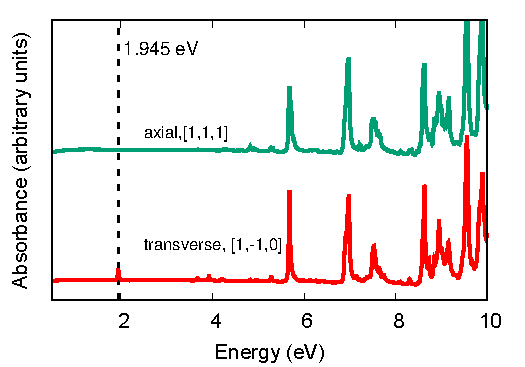
\includegraphics[width=0.5\columnwidth]{Figs/out-NV_spin-polar.pdf}  &
	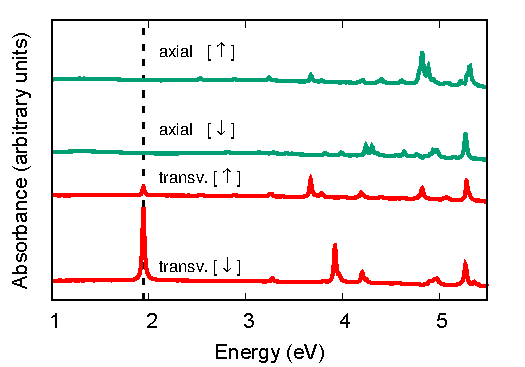
\includegraphics[width=0.5\columnwidth]{Figs/out-NV_spin-polar-zoom.pdf}  \\
	a) & b) 
\end{tabular}
\caption{\footnotesize
Polarization and spin selectivity of the NV$^-$ defect optical response
from spin-collinear RT-TDDFT for the 512-site NV-$x4$ supercell.
(a) Spin-summed spectra for axial and transverse light polarizations.
The axial spectrum corresponds to a kick polarized parallel to the NV
axis, $\mathbf{E}\parallel[111]$, while the transverse spectrum
corresponds to $\mathbf{E}\parallel[1\bar{1}0]$, perpendicular to the
NV axis.  The dashed vertical line marks the experimental NV$^-$
zero-phonon-line energy, $E_{\mathrm{ZPL}}=1.945$~eV.  The
defect-associated peak near this energy is strongly enhanced for
transverse polarization and suppressed for axial polarization,
consistent with the $C_{3v}$ selection rule for the
${}^3A_2\rightarrow{}^3E$ transition.
(b) Expanded view of the sub-gap optical response below approximately
5.5~eV, corresponding to the transparency window of pristine diamond.
In this energy range, optical features arise from the NV$^-$ defect
states rather than from intrinsic band-to-band absorption of the
diamond host.  The spin-resolved spectra show that the transverse
response near the ZPL energy is dominated by the spin-down,
minority-spin channel, consistent with the dominant
$a_1\rightarrow e$ defect excitation shown schematically in
Fig.~\ref{fig:nv-structure}.  The spectra are vertically shifted for
clarity.
}
\label{fig:nv-selection-rules}
\end{figure}

%%%%%%%%%%%%%%%%%%%%%%%%%%%%%%%%%%%%%%%
\subsubsection{Active-space convergence of the defect excitation}

The selection-rule analysis above used the medium-size single-defect
NV-$x4$ supercell at the $\Gamma$ point  with  the TDDFT active space
including full occupied  orbitals  manifold and 3200 virtual orbitals.  
Here we use the same system and transverse polarization %, $\mathbf{E}\parallel[1\bar{1}0]$,
to examine how the defect-associated peak depends on the active
propagation manifold used in the RT-TDDFT calculation.  
%This is an important numerical issue for large-scale real-time simulations.  
As the system size increases, the number of occupied and unoccupied
Kohn--Sham states included in the density-matrix propagation can grow
rapidly, making the computational cost prohibitive.  
Similarly, one might expect the low-energy defect excitation to be only
weakly sensitive to deep occupied states or to high-energy virtual 
states, since the relevant NV$^-$ defect states are localized in the diamond
band gap. We investigate the effect of the TDFFT active space construction on  
position of the experimental zero phonon line  1.945 eV peak to quantify 
the effects of this effect numerically in terms of fraction of the occupied orbitals,
$f_{\mathrm{occ}}= \frac{N_{\mathrm{occ}}^{\mathrm{act}}} {N_{\mathrm{occ}}^{\mathrm{full}}},$
and  the number of virtual states per diamond site,
 $n_{\mathrm{virt}} = \frac{N_{\mathrm{virt}}}{N_{\mathrm{site}}}$, 
 used to construct the TDDFT active space.
Here, $N_{\mathrm{occ}}^{\mathrm{full}}$ represents the total number
of  occupied orbitals, $N_{\mathrm{occ}}^{\mathrm{act}}$ is the number 
of occupied states retained in the propagation, 
 $N_{\mathrm{virt}}$ is the number of unoccupied states included
in the active manifold and $N_{\mathrm{site}}$ is the total number of
diamond lattice sites before formation of the defect.

For the 512-site NV-$x4$ supercell used in this convergence test,
$N_{\mathrm{occ}}^{\mathrm{full}}=1024$ and $N_{\mathrm{site}}=512$.
The occupied-space tests removed the lowest 0, 200, 400, 512, 600, and
800 occupied Kohn--Sham states from the active propagation manifold.
This corresponds to retaining 1024, 824, 624, 512, 424, and 224
occupied states, or approximately 100\%, 80\%, 60\%, 50\%, 40\%, and
20\% of the occupied manifold, respectively.  The virtual-space tests
used $N_{\mathrm{virt}}=512$, 1024, 2048, and 3200, corresponding to
$n_{\mathrm{virt}}=1$, 2, 4, and 6.25 virtual states per diamond site.

Figure~\ref{fig:nv-active-space} shows the effect of  occupied- and
virtual-space truncation  on the position  of the
defect-associated peak near the experimental ZPL energy.  Reducing
$f_{\mathrm{occ}}$ shifts the peak to higher energy, showing that the
deep occupied manifold cannot be discarded without changing the
computed defect excitation.  Conversely, increasing
$n_{\mathrm{virt}}$ systematically shifts the peak to lower energy,
with the peak position approaching a saturated value as the virtual
space is enlarged.  
%Thus, although the dominant excitation has a
%localized $a_1\rightarrow e$ character, the computed transition energy
%is not converged by a minimal defect-only active space.
Physically, this behavior indicates that the localized defect
excitation is dressed by the polarizable diamond environment and by the
self-consistent time-dependent response of the electron density.
Truncating either the occupied or unoccupied part of the propagation
manifold suppresses electronic relaxation and screening around the
particle-hole excitation, producing a measurable blueshift 



%--------------------------------------------------------------------------------
\begin{figure}[ht!]
\centering
%\includegraphics[width=\columnwidth]{Figs/out-NV-active-space.pdf}
%See the figure here: /Users/j2c/ORNL Dropbox/Jacek Jakowski/Projects-current/LDRD-2025-NEAT-spin-dynamics/NV-center/Spectra/Debug
\begin{tabular}{ll}
	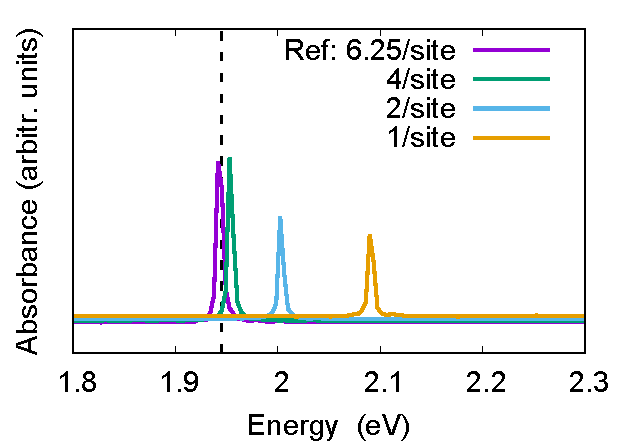
\includegraphics[width=0.5\columnwidth]{Figs/out-nv-x4_nocc.pdf} &
        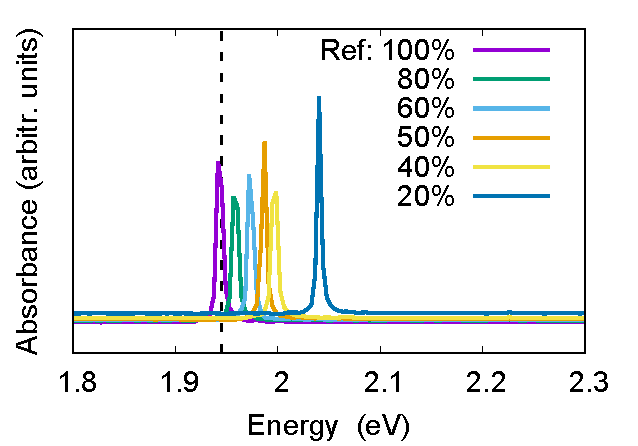
\includegraphics[width=0.5\columnwidth]{Figs/out-nv-x4_start_state.pdf}  \\ 
	a) & b) 
\end{tabular}
%\caption{\footnotesize
%Active-space convergence of the defect-associated optical response for
%the 512-site NV-$x4$ supercell at the $\Gamma$ point, using transverse
%polarization $\mathbf{E}\parallel[1\bar{1}0]$.  The spectra are obtained
%from the Fourier transform of the time-dependent current response and
%are shown as absorbance in arbitrary units.  The dashed vertical line
%marks the experimental NV$^-$ zero-phonon-line energy,
%$E_{\mathrm{ZPL}}=1.945$~eV.  (a) Dependence on the retained occupied
%fraction,
%$f_{\mathrm{occ}}=N_{\mathrm{occ}}^{\mathrm{act}}/
%N_{\mathrm{occ}}^{\mathrm{full}}$.  For this 512-site supercell,
%$N_{\mathrm{occ}}^{\mathrm{full}}=1024$; the calculations removed the
%lowest 0, 200, 400, 512, 600, and 800 occupied states, corresponding
%approximately to retaining 100\%, 80\%, 60\%, 50\%, 40\%, and 20\% of
%the occupied manifold.  Reducing the occupied active space shifts the
%defect-associated peak to higher energy.  (b) Dependence on the virtual
%active space, expressed as the number of virtual states per diamond
%site, $n_{\mathrm{virt}}=N_{\mathrm{virt}}/N_{\mathrm{site}}$.  The
%values $n_{\mathrm{virt}}=1$, 2, 4, and 6.25 correspond to
%$N_{\mathrm{virt}}=512$, 1024, 2048, and 3200 for the 512-site cell.
%Increasing the virtual active space systematically red-shifts the peak
%toward a saturated value, demonstrating that the localized defect
%excitation is dressed by the electronic response of the surrounding
%diamond host. 
%}
%\label{fig:nv-active-space}
%
\caption{\footnotesize
Active-space convergence of the defect-associated optical response for
the 512-site NV-$x4$ supercell at the $\Gamma$ point, using transverse
polarization along $[1\bar{1}0]$ direction.  
%The spectra are obtained from the Fourier transform of the time-dependent current response and
%are shown as absorbance in arbitrary units.  
The dashed vertical line marks the experimental NV$^-$ zero-phonon-line energy,
$E_{\mathrm{ZPL}}=1.945$~eV.  The reference calculation, shown in both
panels, uses the full occupied space, $f_{\mathrm{occ}}=100\%$, and 
$N_{\mathrm{virt}}=3200$, corresponding to $n_{\mathrm{virt}}=6.25$ virtual states
per diamond site for the 512-site cell. 
(a) Dependence on the virtual active space, expressed as the number of
virtual states per diamond site,
$n_{\mathrm{virt}}=N_{\mathrm{virt}}/N_{\mathrm{site}}$.  The values
$n_{\mathrm{virt}}=1$, 2, 4, and 6.25 correspond to
$N_{\mathrm{virt}}=512$, 1024, 2048, and 3200, respectively.
Increasing $n_{\mathrm{virt}}$ systematically red-shifts the peak
toward a saturated value.
(b) Dependence on the retained occupied fraction,
$f_{\mathrm{occ}}=N_{\mathrm{occ}}^{\mathrm{act}}/
N_{\mathrm{occ}}^{\mathrm{full}}$.  
The retained values  100\%, 80\%, 60\%, 50\%, 40\%, and 20\% are approximate 
and correspond to 1024, 800, 600, 512, 400, and 200 occupied states.
%$N_{\mathrm{occ}}^{\mathrm{full}}=1024$; the tested values correspond
%to removing the lowest 0, 200, 400, 512, 600, and 800 occupied states,
%or retaining approximately 100\%, 80\%, 60\%, 50\%, 40\%, and 20\% of
%the occupied space.  
Reducing $f_{\mathrm{occ}}$ shifts the defect-associated peak to higher energy.
}
\label{fig:nv-active-space}
\end{figure}

%--------------------------------------------------------------------------------
Furthemore, the two convergence tests show different sensitivities.  At fixed
$n_{\mathrm{virt}}=6.25$, reducing the retained occupied fraction from
100\% to about 50\% produces only a modest blue shift of the
defect-associated peak, while retaining only about 20\% of the occupied
space leads to a larger shift.  By contrast, at fixed
$f_{\mathrm{occ}}=100\%$, increasing the virtual active space from
$n_{\mathrm{virt}}=1$ to 4--6.25 virtual states per site produces a
substantially larger red shift and brings the peak close to the
experimental ZPL energy.  Thus, for this NV-$x4$ test case, the
unoccupied portion of the active space is the primary convergence
bottleneck for the peak position, while the occupied manifold can be
moderately truncated with a smaller, but still measurable, effect.

In summary, the peak position is more sensitive to the size of the virtual active
space than to moderate truncation of the occupied manifold.  However,
aggressive occupied-space truncation also produces a measurable blue
shift, indicating that the response of deeper valence states contributes
to the screening and relaxation of the localized defect excitation.




%%%%%%%%%%%%%%%%%%%%%%%%%%%%%%%%%%%%%%%%%%%%
\subsubsection{Defect concentration and magnetic alignment in
replicated NV$^-$ arrays}
\label{sec:nv-arrays}

The large NV-$x8$ supercell also provides a controlled framework for
examining how the optical response evolves with defect concentration.
Starting from the same 4096-site diamond host, we constructed cells
containing 1, 8, and 64 NV$^-$ centers.  These systems correspond,
respectively, to the defect concentrations obtained from the NV-$x8$,
NV-$x4$, and NV-$x2$ cells: the 8-NV structure is generated by a
$2\times2\times2$ replication of the NV-$x4$ cell, whereas the 64-NV
structure is generated by a $4\times4\times4$ replication of the
NV-$x2$ cell.  The comparison therefore changes the number and
separation of the defects while retaining the same total supercell
size, real-space grid, transverse field polarization, spectral
broadening, and $\Gamma$-point representation.  The concentration
series discussed first uses a parallel collinear alignment of the NV
moments.

The RT-TDDFT calculations for the three 4096-site systems also used
the same active-space density.  Approximately $67\%$ of the occupied
space was retained, while the virtual space contained approximately
two unoccupied states per diamond site.  In the RMG state-count
convention, the calculations used 16400 computed states, with 2700
deep occupied states frozen and four highest-energy states discarded,
leaving 13696 states in the density-matrix propagation.  Each spectrum
was obtained from 42000 electronic time steps with
$\Delta t=1.0$~a.u., corresponding to a total propagation time of
approximately 1.02~ps.  Consequently, differences among the three
RT-TDDFT spectra predominantly reflect the NV concentration rather
than changes in total cell size, propagation length, or active-space
density.

For comparison, we also evaluated the optical response within the
independent-particle approximation (IPA) using the
\texttt{LOPTICS} implementation in RMG.  In atomic units, the
spin-resolved imaginary part of the IPA dielectric tensor can be
written as
%
\begin{equation}
\epsilon_{\alpha\beta}^{(2),\sigma}(\omega)
=
\frac{4\pi^2}{\Omega\omega^2}
\sum_{\mathbf{k}} w_{\mathbf{k}}
\sum_{v,c}
\left(
f_{v\mathbf{k}\sigma}-f_{c\mathbf{k}\sigma}
\right)
\operatorname{Re}
\left[
P_{vc\mathbf{k}\sigma}^{\alpha *}
P_{vc\mathbf{k}\sigma}^{\beta}
\right]
\delta_{\eta}
\left(
\epsilon_{c\mathbf{k}\sigma}
-\epsilon_{v\mathbf{k}\sigma}
-\omega
\right),
\label{eq:nv-ipa}
\end{equation}
%
where $\Omega$ is the supercell volume, $w_{\mathbf{k}}$ is the
$\mathbf{k}$-point weight, and $P_{vc\mathbf{k}\sigma}^{\alpha}$ is
the velocity-gauge transition matrix element, including the
nonlocal-pseudopotential contribution.  The indices $v$ and $c$
denote occupied and unoccupied Kohn--Sham states of the same global
spin $\sigma$, and $\delta_{\eta}$ represents the broadened
energy-conservation condition.  The IPA spectra therefore expose the
underlying vertical Kohn--Sham transition structure, whereas the
RT-TDDFT spectra additionally contain the self-consistent induced
Hartree and adiabatic exchange--correlation response.  The IPA curves
in Fig.~\ref{fig:nv-concentration-ipa} were independently scaled for
clarity, so the comparison concerns peak positions and spectral
structure rather than absolute intensities.

Figure~\ref{fig:nv-concentration-ipa} shows a pronounced evolution of
the optical response with decreasing NV concentration.  For the
64-NV array, corresponding to the NV-$x2$ concentration, both IPA and
RT-TDDFT produce strongly fragmented spectra over the sub-gap energy
range.  The large number of optically active features is consistent
with substantial coupling among the closely spaced defects, which
hybridizes the defect-derived states and produces dispersive
occupied and unoccupied defect bands.  The NV-$x2$ concentration is
therefore clearly outside the isolated-defect regime.

At the intermediate NV-$x4$ concentration, represented by eight
defects in the same 4096-site host, the spectral response becomes much
simpler.  The IPA spectrum retains several closely spaced transitions
in the vicinity of the experimental ZPL energy, indicating that some
fine structure remains in the underlying Kohn--Sham transition
spectrum.  By contrast, the self-consistent RT-TDDFT response is
dominated by a single resonance near 2.01~eV.  This simplification is
consistent with coupling and redistribution of oscillator strength
among nearby independent-particle transitions in the time-dependent
response.  Finite spectral resolution and the truncated RT-TDDFT
active space may also suppress weaker components, so the single
RT-TDDFT peak should not be interpreted as evidence that every
periodic-image effect has disappeared.  Nevertheless, it shows that
the dominant optical observable is already substantially
single-resonance-like at the NV-$x4$ defect separation.

Further dilution to a single NV$^-$ center in the 4096-site NV-$x8$
cell produces a similarly simple low-energy response.  The qualitative
similarity of the dominant RT-TDDFT peaks for the 8-NV and 1-NV
systems supports the conclusion that a separation corresponding to the
512-site NV-$x4$ model is sufficient to recover the principal
defect-associated optical feature within the present spectral
resolution and active-space approximation.  The calculated peak near
2.01~eV remains approximately 0.06~eV above the experimental
1.945-eV ZPL.  As shown by the active-space analysis in
Sec.~\ref{sec:nv-active-space}, part of this residual blueshift is
consistent with the restricted occupied and virtual propagation
spaces used for the 4096-site calculations.  The experimental ZPL is
nevertheless used only as a reference because the present frozen-ion
adiabatic-PBE response also omits excited-state structural relaxation
and vibronic effects.



%-rw-r--r--@ 1 j2c  staff   450123 Jul 14 18:43 Figure-nv-AFM-FM.pdf
%-rw-r--r--@ 1 j2c  staff  2947596 Jul 14 18:46 Figure-nv-AFM-FM.pptx
%-rw-r--r--@ 1 j2c  staff    52351 Jul 14 20:20 out-nv-supercell_eV.pdf

\begin{figure}[ht!]
    \centering
    % Replace the filename below with the final figure filename.  IPA
	\begin{tabular}{ll}
		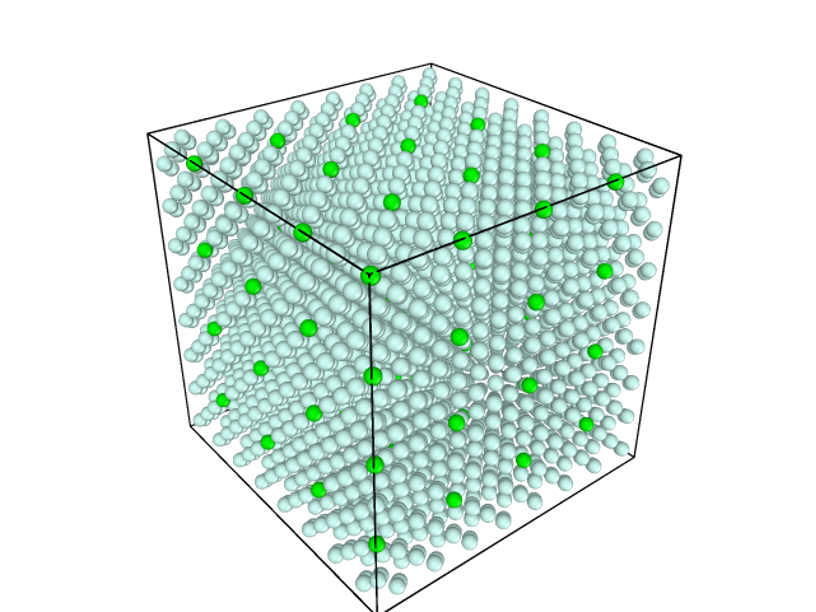
\includegraphics[width=0.4\linewidth]{Figs/nv-model-64-centers.png} &
		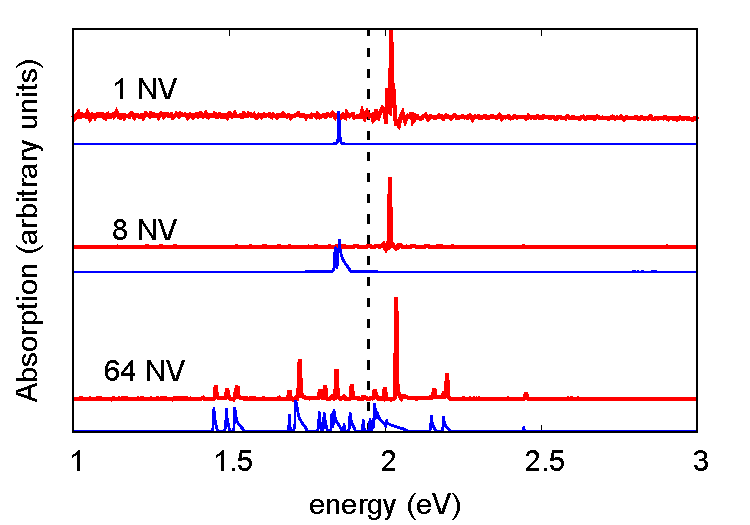
\includegraphics[width=0.5\linewidth]{Figs/out-nv-supercell_eV.pdf} \\
		a) & b)
	\end{tabular}
    \caption{\footnotesize
    Concentration dependence of the optical response in parallel-aligned
    NV$^-$ arrays.  Spin-collinear RT-TDDFT spectra are shown in red and
    independent-particle approximation (IPA) spectra, evaluated with the
    \texttt{LOPTICS} implementation in RMG, are shown in blue.  From top
    to bottom, the systems contain 1, 8, and 64 NV$^-$ centers in the
    same 4096-site diamond host, corresponding to the NV-$x8$, NV-$x4$,
    and NV-$x2$ defect concentrations, respectively.  All calculations
    use the same atomic structures, real-space grid, $\Gamma$-point
    representation, transverse polarization, and spectral broadening.
    The RT-TDDFT calculations additionally use the same retained
    occupied fraction and number of virtual states per diamond site and
    were propagated for 42000 steps with $\Delta t=1.0$~a.u.,
    corresponding to approximately 1.02~ps.  The dashed vertical line
    marks the experimental zero-phonon-line energy,
    $E_{\mathrm{ZPL}}=1.945$~eV.  The strongly fragmented spectrum of
    the 64-NV array reflects substantial coupling among closely spaced
    defects.  At the 8-NV concentration, the IPA retains nearby
    independent-particle transition structure, whereas the RT-TDDFT
    response is dominated by a single resonance resembling that of the
    dilute single-NV system.  The spectra are vertically offset, and
    the IPA curves are independently scaled, for clarity.}
    \label{fig:nv-concentration-ipa}
\end{figure}

The fixed-volume replicated cells also permit examination of how the
magnetic arrangement of the NV moments affects the spin-resolved
optical response.  We considered both a parallel collinear
configuration, denoted FM below, and a G-type antiparallel
broken-symmetry configuration, denoted G-AFM, for the 64-NV and 8-NV
arrays.  In the FM configuration, all local defect moments are aligned
with the same global spin axis.  In the G-AFM configuration, the local
moment orientation alternates between neighboring defect sites.

The persistence of the local moments in these configurations can be
characterized using the total and absolute magnetizations,
%
\begin{equation}
M_{\mathrm{tot}}
=
\mu_{\mathrm B}
\int
\left[
\rho_{\uparrow}(\mathbf r)-\rho_{\downarrow}(\mathbf r)
\right]d\mathbf r,
\qquad
M_{\mathrm{abs}}
=
\mu_{\mathrm B}
\int
\left|
\rho_{\uparrow}(\mathbf r)-\rho_{\downarrow}(\mathbf r)
\right|d\mathbf r.
\label{eq:nv-magnetization}
\end{equation}
%
For the 8-NV array, the FM solution gives
$M_{\mathrm{tot}}=20.73~\mu_{\mathrm B}$ and
$M_{\mathrm{abs}}=22.36~\mu_{\mathrm B}$, whereas the G-AFM solution
gives $M_{\mathrm{tot}}=0$ and
$M_{\mathrm{abs}}=18.66~\mu_{\mathrm B}$.  The corresponding values
for the 64-NV array are
$M_{\mathrm{tot}}=128.42~\mu_{\mathrm B}$ and
$M_{\mathrm{abs}}=143.03~\mu_{\mathrm B}$ for the FM arrangement, and
$M_{\mathrm{tot}}=0$ and
$M_{\mathrm{abs}}=138.57~\mu_{\mathrm B}$ for the G-AFM arrangement.
The vanishing total magnetization but substantial absolute
magnetization of the G-AFM solutions confirms that the local defect
moments remain present and cancel globally rather than disappearing.

The spin-resolved spectra in Fig.~\ref{fig:nv-fm-gafm} show how the
local minority-spin selection rule established for the single NV
center maps onto the globally defined spin channels of a multi-defect
array.  In the FM configuration, all local moments have the same
orientation.  The local minority-spin $a_1\rightarrow e$ excitation
therefore corresponds to the same global spin channel at every defect,
and the optical response is strongly dominated by one spin component.
In the G-AFM arrangement, the local moment is reversed on the second
magnetic sublattice.  The local minority-spin excitation consequently
maps onto one global spin channel on one sublattice and the opposite
global spin channel on the other.  The corresponding defect-associated
features therefore appear in both global spin-resolved spectra.

This redistribution between global spin channels does not represent a
spin-flip optical transition.  The optical perturbation remains spin
independent and the transitions conserve the global collinear spin
label.  Instead, the result reflects the reversal of the local moment
relative to the fixed global quantization axis.  Local minority spin is
represented by opposite global spin labels on the two G-AFM
sublattices.

The concentration dependence found above is also evident in the
magnetic comparison.  At the NV-$x2$ concentration, both FM and G-AFM
spectra contain many defect-associated peaks, and the detailed
distribution of these features depends on the magnetic arrangement.
At the more dilute NV-$x4$ concentration, the response is concentrated
primarily in a single resonance near 2.0~eV.  Changing from FM to
G-AFM then affects mainly the distribution of this resonance between
the two global spin channels rather than producing a comparably strong
fragmentation of the spectrum.  This behavior is consistent with a
substantial reduction of electronic coupling among the NV centers as
their separation increases.

\begin{figure}[ht!]
    \centering
    % Replace the filename below with the final figure filename.
		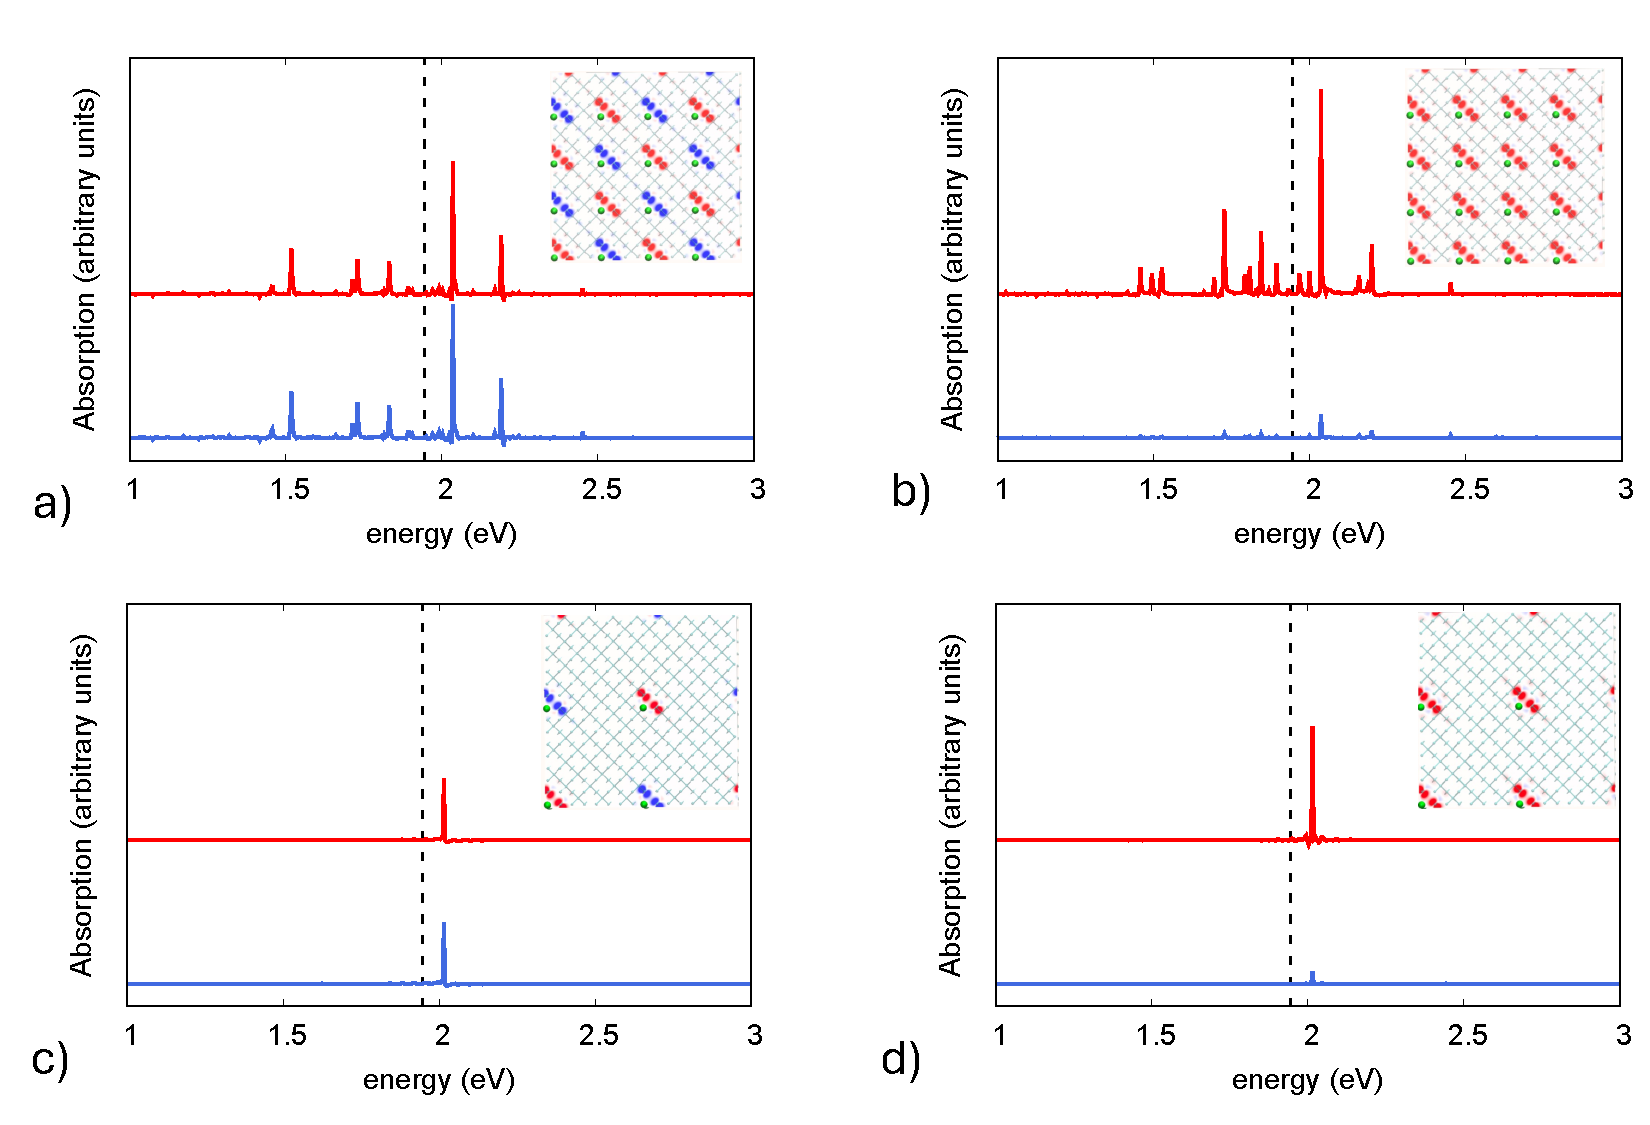
\includegraphics[width=0.9\linewidth]{Figs/Figure-nv-AFM-FM.pdf} 
    \caption{\footnotesize
    Spin-resolved RT-TDDFT optical response of replicated NV$^-$ arrays
    in the 4096-site diamond host.  The upper row shows the
    64-NV system at the NV-$x2$ concentration, and the lower row shows
    the 8-NV system at the NV-$x4$ concentration.  Panels (a) and (c)
    correspond to G-type antiparallel broken-symmetry arrangements,
    whereas panels (b) and (d) correspond to parallel, FM
    arrangements.  The red and blue curves show the two globally
    defined collinear spin channels and are vertically offset for
    clarity.  The insets illustrate the corresponding local defect-spin
    arrangements; red and blue markers denote opposite local moment
    orientations.  The dashed vertical lines mark the experimental
    NV$^-$ zero-phonon-line energy,
    $E_{\mathrm{ZPL}}=1.945$~eV.  In the FM configurations, the local
    minority-spin defect excitation maps predominantly onto one global
    spin channel.  In the G-AFM configurations, reversal of the local
    moments between the two magnetic sublattices causes the same local
    minority-spin excitation to appear in both global spin channels.
    The response remains strongly fragmented at the NV-$x2$
    concentration but becomes predominantly single-resonance-like at
    the NV-$x4$ concentration.}
    \label{fig:nv-fm-gafm}
\end{figure}

Together, these calculations show that increasing the NV--NV
separation transforms the optical response from the fragmented
spectrum of an interacting defect array to a dominant
isolated-defect-like resonance.  At the same time, the magnetic
alignment determines how the local minority-spin excitation is
represented in the globally defined spin channels.  The 4096-site
calculations therefore demonstrate that the periodic spin-collinear
RT-TDDFT implementation can treat both dilute defects and extended
arrays containing as many as 64 optically active defect centers within
the same real-space simulation framework.


